% !Mode:: "TeX:UTF-8"

\chapter{前端项目}

\section{项目需求}

前端项目是第二阶段,使用HTML+CSS+JS技术开发企业级静态网页,完成后续项目中前端部分的布局。使用HTML技术完成前端静态网页应用程序的实现,使用CSS技术对网页进行样式渲染,使用JavaScript语言制作网页特效。

\subsection{首页功能}
\subsubsection*{\normalsize主要功能}
显示点餐分类信息
\subsubsection*{\normalsize动作}
1.点击点餐分类小图片,跳转到商家列表页面

2.点击下方菜单栏中的“订单”,跳转到历史订单页面
\begin{figure}[H]
    \centering
    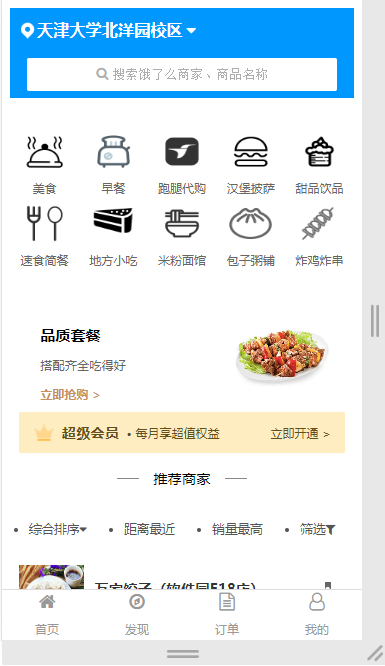
\includegraphics[width=5.4cm,height=9.6cm]{figures/2.2.1.png}
    \caption{首页功能}
\end{figure}

\subsection{商家列表页面功能}
\subsubsection*{\normalsize主要功能}
显示商家列表信息
\subsubsection*{\normalsize动作}
点击某个商家,跳转到此商家的详细信息页面
\begin{figure}[H]
    \centering
    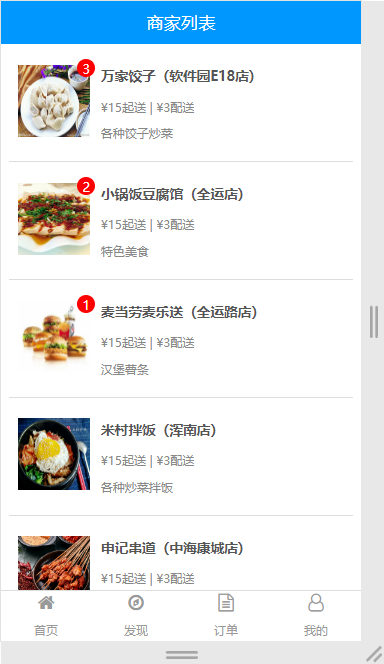
\includegraphics[width=5.4cm,height=9.6cm]{figures/2.2.2.png}
    \caption{商家列表页面功能}
\end{figure}

\subsection{商家详细信息页面功能}
\subsubsection*{\normalsize主要功能}
显示商家详细信息及所属食品信息
\subsubsection*{\normalsize动作}
点击“去结算”按钮,跳转到确认订单页面
\begin{figure}[H]
    \centering
    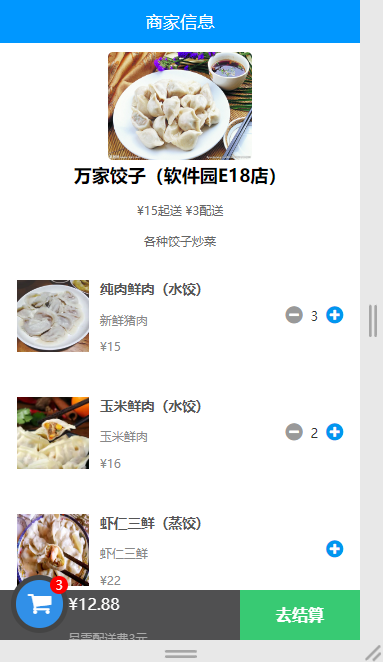
\includegraphics[width=5.4cm,height=9.6cm]{figures/2.2.3.png}
    \caption{商家详细信息页面功能}
\end{figure}

\subsection{确认订单页面功能}
\subsubsection*{\normalsize主要功能}
1.显示订单信息

2.选择送货地址
\subsubsection*{\normalsize动作}
1.点击送货地址,跳转到送货地址列表页面

2.点击“去支付”按钮,跳转到支付页面
\begin{figure}[H]
    \centering
    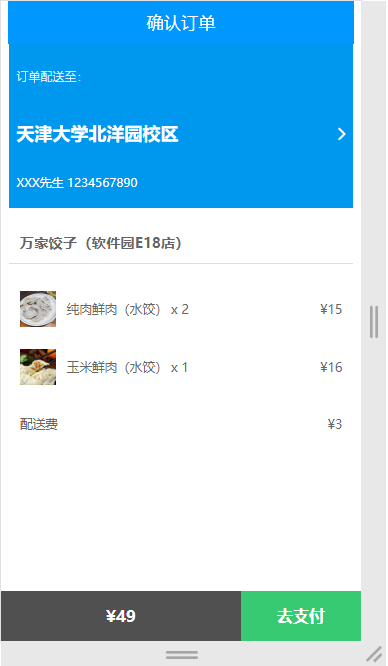
\includegraphics[width=5.4cm,height=9.6cm]{figures/2.2.4.png}
    \caption{确认订单页面功能}
\end{figure}

\subsection{在线支付页面功能}
\subsubsection*{\normalsize主要功能}
显示订单信息及订单明细信息
\subsubsection*{\normalsize动作}
无
\begin{figure}[H]
    \centering
    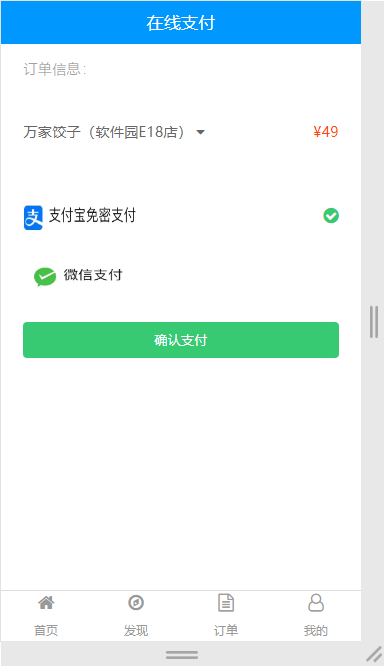
\includegraphics[width=5.4cm,height=9.6cm]{figures/2.2.5.png}
    \caption{在线支付页面功能}
\end{figure}

\subsection{登录页面功能}
\subsubsection*{\normalsize主要功能}
用户登录
\subsubsection*{\normalsize动作}
1.点击“登陆”按钮,跳转到上一个页面

2.点击“去注册”按钮,跳转到注册页面
\begin{figure}[H]
    \centering
    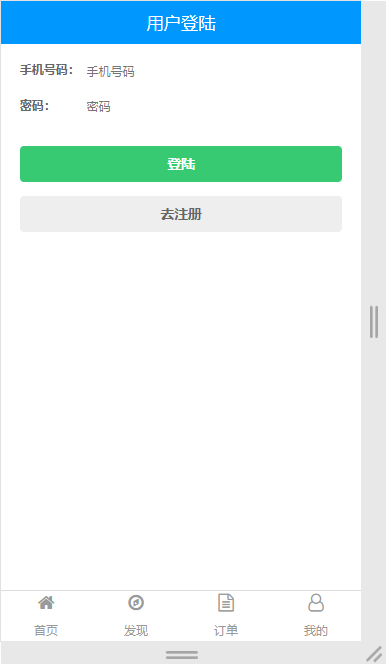
\includegraphics[width=5.4cm,height=9.6cm]{figures/2.2.6.png}
    \caption{登录页面功能}
\end{figure}

\subsection{注册页面功能}
\subsubsection*{\normalsize主要功能}
注册新用户
\subsubsection*{\normalsize动作}
点击“注册”按钮,跳转到登陆页面
\begin{figure}[H]
    \centering
    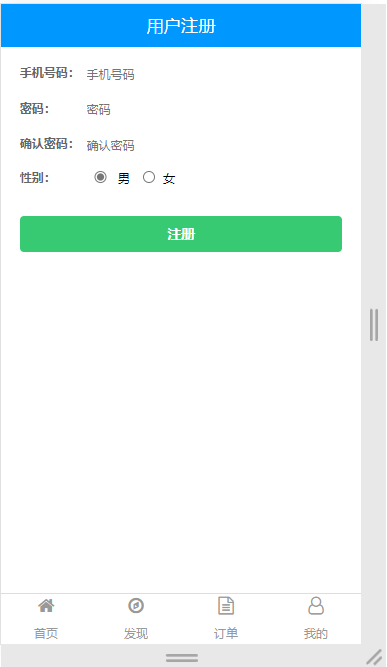
\includegraphics[width=5.4cm,height=9.6cm]{figures/2.2.7.png}
    \caption{注册页面功能}
\end{figure}

\subsection{历史订单页面功能}
\subsubsection*{\normalsize主要功能}
显示用户历史订单信息
\subsubsection*{\normalsize动作}
点击某个历史订单,可以对订单明细信息进行显示和隐藏
\begin{figure}[H]
    \centering
    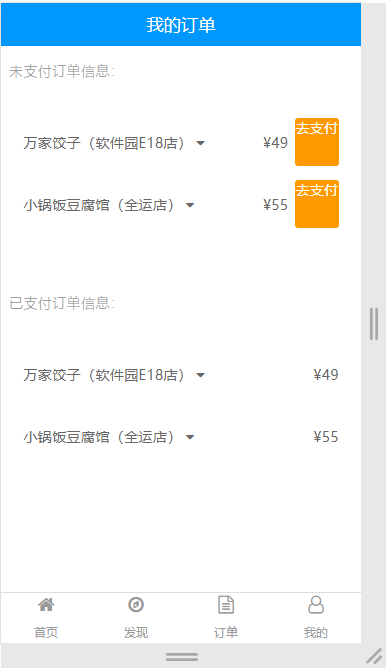
\includegraphics[width=5.4cm,height=9.6cm]{figures/2.2.8.png}
    \caption{历史订单页面功能}
\end{figure}

\section{项目设计}
\subsection{移动端网页设计}
\subsubsection*{\normalsize问题}
移动端屏幕尺寸多变,不像PC端屏幕那样统一。这样就造成在移动端显示网页时,由于尺寸问题,会出现显示不下
网页,从而出现横向滚动条现象。 为了解决这个问题,出现了viewport(屏幕视口)的概念。
\subsubsection*{\normalsize解决方案}
使用viewport解决上述问题。先将网页放入layout viewport中,然后在将layout viewport等比例缩小到ideal viewport中。这样就能保证:无论什么样的网页,都能在手机屏幕上显示,而且没有横向滚动条。

\subsection{弹性布局}
\subsubsection*{\normalsize概念:主轴和侧轴}
弹性布局中的一个重要概念:主轴与侧轴: 弹性盒子中默认存在两根轴,一个是水平方向的主轴,一个是垂直方向的侧轴。
\begin{figure}[H]
    \centering
    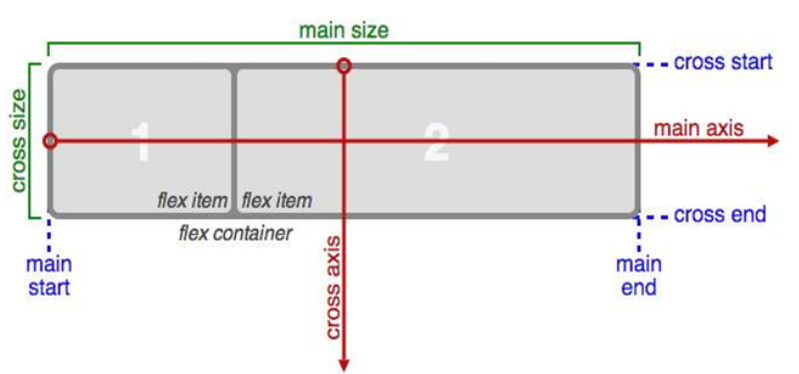
\includegraphics[scale=0.7]{figures/2.2.9.png}
    \caption{主轴和侧轴}
\end{figure}

\subsubsection*{\normalsize设计方法}
1.使用flex-direction属性设置主轴方向。

2.使用flex-wrap:wrap让子元素自动换行。

3.设置align-items样式。常用值有三种:flex-start(上对齐)、flex-end(下对齐)、center(居中)。

4.使用flex给子元素分配空间,从而让每个子元素所占空间不一致。

\subsection{视口尺寸}
视口:在PC端,指浏览器的可视区域;在移动端,指Viewport 中的 Layout Viewport。 视口尺寸常用的有以下2
个: vw : 1vw 等于视口宽度的1\% vh : 1vh 等于视口高度的1\% 实际应用中,可以使用vw,实现元素宽度和高度成
比例自动缩放。

\subsection{边框盒子模型}
CSS3之前的盒子模型,可以说是content-box型盒子,即宽和高为内容。 CSS3之后新增了一的盒子模型,可以说
是border-box型盒子,即宽和高为边框。 那么,使用box-sizing属性可以设置盒子模型类型。